\begin{figure}[ht!]
  \centering
  \caption{Sectoral carbon intensities from GTAP} \label{fig:GTAP}\label{fig:B}
  \begin{subfigure}[b]{\textwidth}
  \centering
  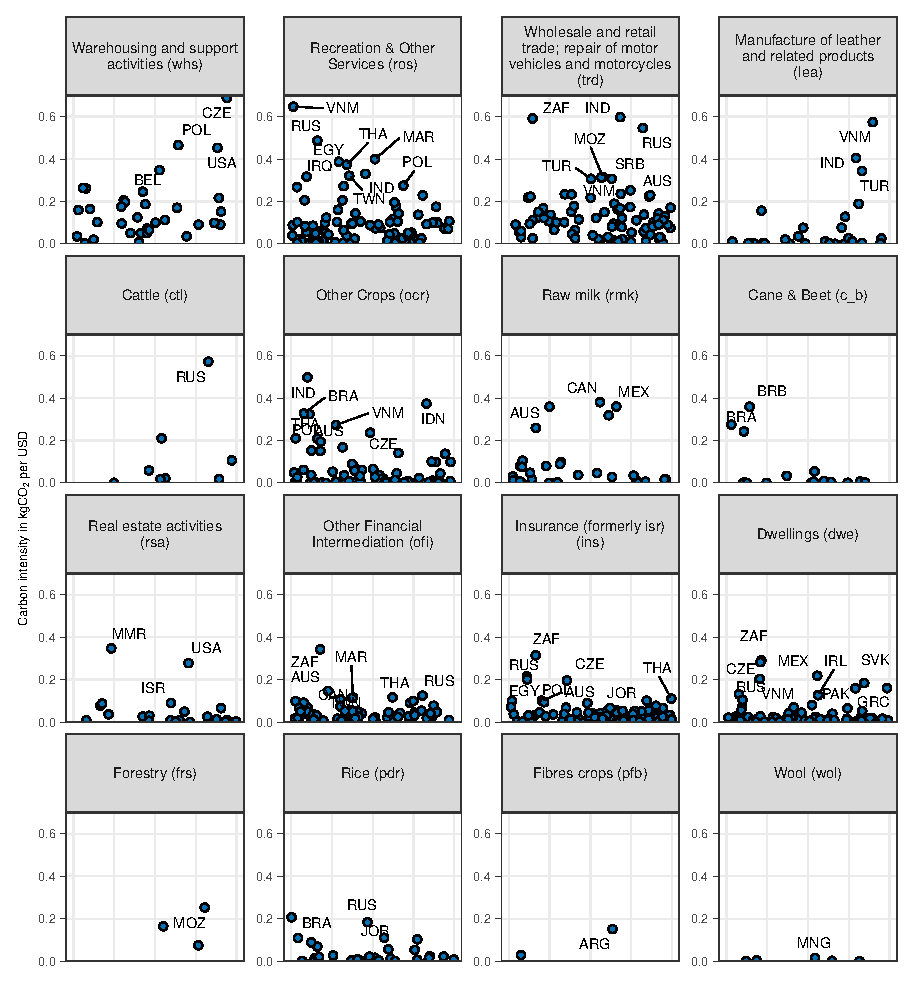
\includegraphics{Analysis_Carbon_Intensities_GTAP/Figure_2.1.1_A_2017B.pdf}
  \caption{Sectoral carbon intensities from GTAP - Part A} \label{fig:B1}  
  \begin{subcaption2}
    This figure displays sectoral carbon intensities in kgCO$_{2}$ per USD of output for 16 sectors. We plot sectoral carbon intensities if household budget surveys in respective countries include consumption items which correspond to each sector. See our online repository for all country- and sector-level carbon intensities. We include labels with country codes if sector outputs are relatively carbon-intensive compared to other countries. Note that sectors \textit{other mining extraction (oxt)}, \textit{construction (cns)} and \textit{extraction of crude petroleum (oil)} are not matched to any item in any country.
  \end{subcaption2}
\end{subfigure}
\end{figure}

\clearpage

\begin{figure}[ht!]\ContinuedFloat
\begin{subfigure}[b]{\textwidth}
  \centering
  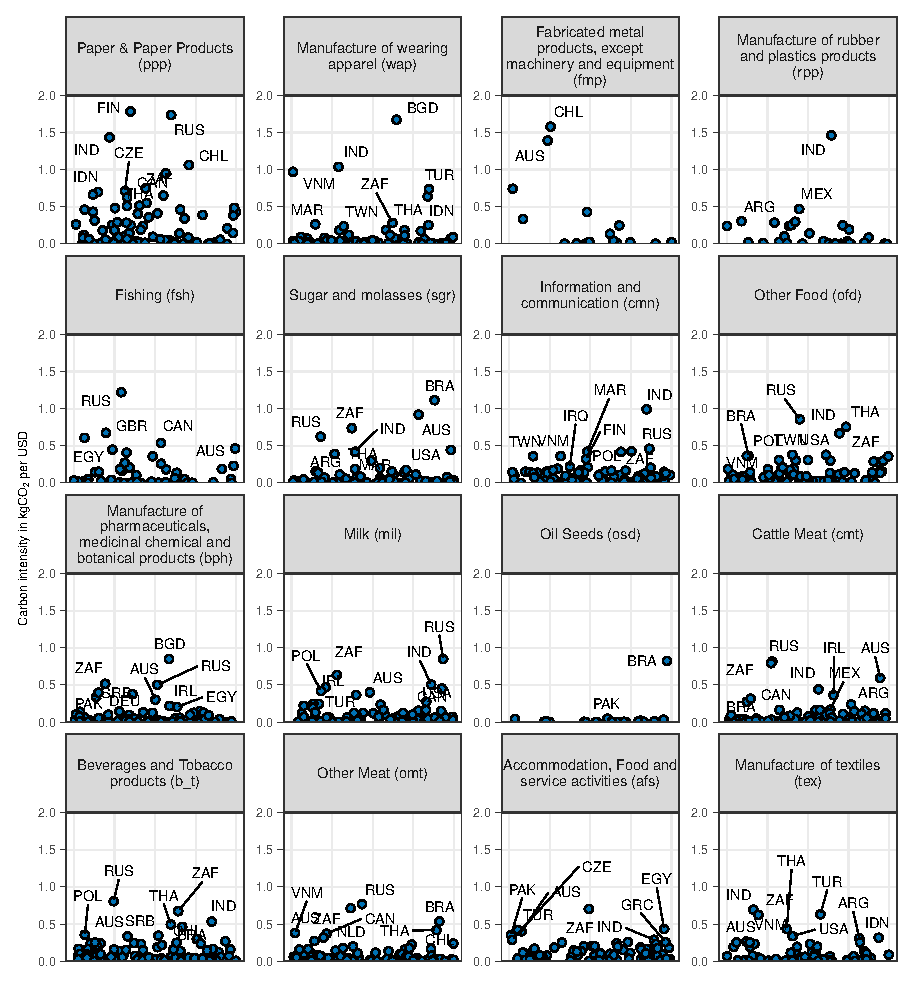
\includegraphics{Analysis_Carbon_Intensities_GTAP/Figure_2.1.1_B_2017B.pdf}
  \caption{Sectoral carbon intensities from GTAP - Part B} \label{fig:B2}  
  \begin{subcaption2}
    This figure displays sectoral carbon intensities in kgCO$_{2}$ per USD of output for 16 sectors. We plot sectoral carbon intensities if household budget surveys in respective countries include consumption items which correspond to each sector. See our online repository for all country- and sector-level carbon intensities. We include labels with country codes if sector outputs are relatively carbon-intensive compared to other countries. Note that sectors \textit{other mining extraction (oxt)}, \textit{construction (cns)} and \textit{extraction of crude petroleum (oil)} are not matched to any item in any country.
  \end{subcaption2}
\end{subfigure}
\end{figure}

\clearpage

\begin{figure}[ht!]\ContinuedFloat
\begin{subfigure}[b]{\textwidth}
  \centering
  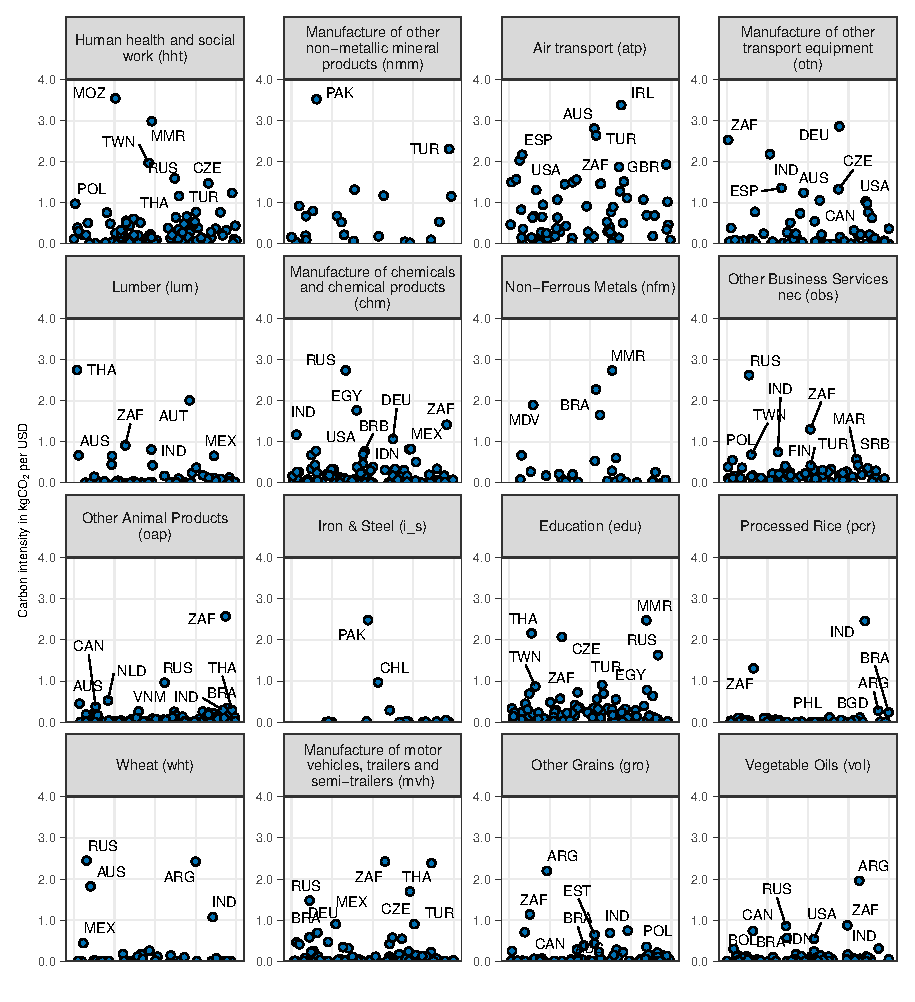
\includegraphics{Analysis_Carbon_Intensities_GTAP/Figure_2.1.1_C_2017B.pdf}
  \caption{Sectoral carbon intensities from GTAP - Part C} \label{fig:B3}  
  \begin{subcaption2}
    This figure displays sectoral carbon intensities in kgCO$_{2}$ per USD of output for 16 sectors. We plot sectoral carbon intensities if household budget surveys in respective countries include consumption items which correspond to each sector. See our online repository for all country- and sector-level carbon intensities. We include labels with country codes if sector outputs are relatively carbon-intensive compared to other countries. Note that sectors \textit{other mining extraction (oxt)}, \textit{construction (cns)} and \textit{extraction of crude petroleum (oil)} are not matched to any item in any country.
  \end{subcaption2}
\end{subfigure}
\end{figure}

\clearpage

\begin{figure}[ht!]\ContinuedFloat
\begin{subfigure}[b]{\textwidth}
  \centering
  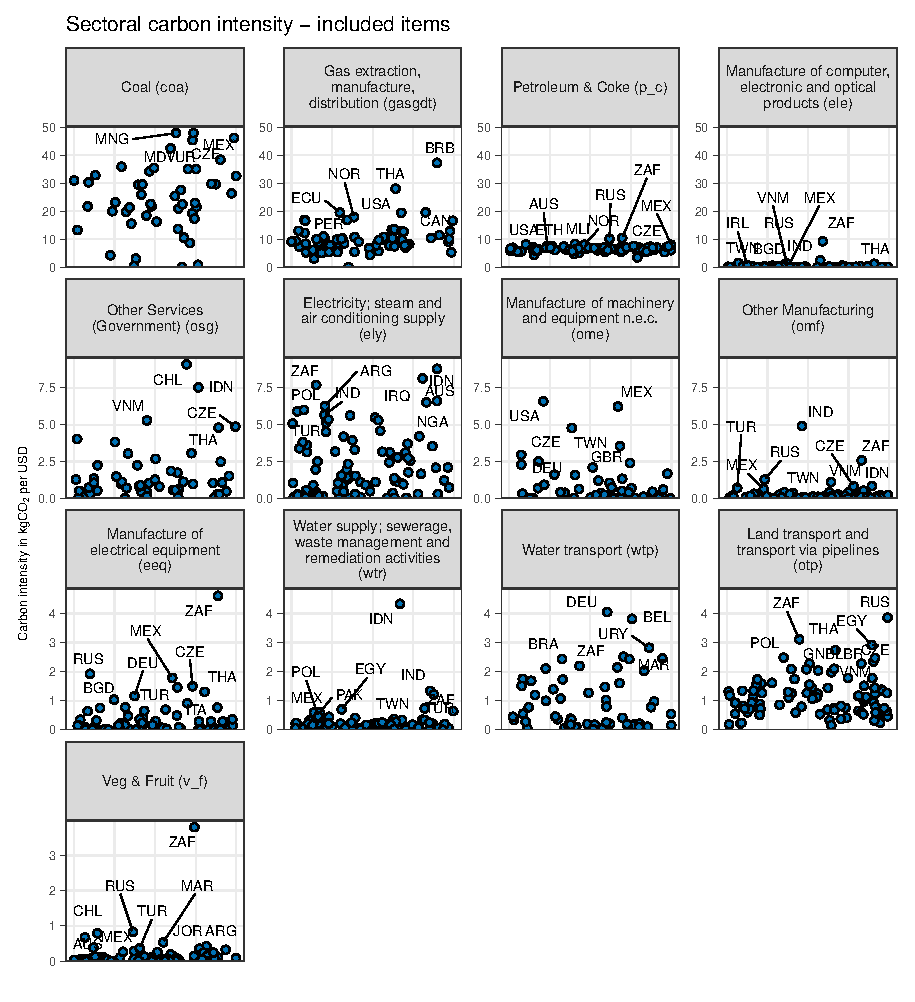
\includegraphics{Analysis_Carbon_Intensities_GTAP/Figure_2.1.1_D_2017B.pdf}
  \caption{Sectoral carbon intensities from GTAP - Part D} \label{fig:B4}  
  \begin{subcaption2}
    This figure displays sectoral carbon intensities in kgCO$_{2}$ per USD of output for 13 sectors. We plot sectoral carbon intensities if household budget surveys in respective countries include consumption items which correspond to each sector. See our online repository for all country- and sector-level carbon intensities. We include labels with country codes if sector outputs are relatively carbon-intensive compared to other countries. Note that sectors \textit{other mining extraction (oxt)}, \textit{construction (cns)} and \textit{extraction of crude petroleum (oil)} are not matched to any item in any country.
  \end{subcaption2}
\end{subfigure}
\end{figure}

\clearpage